\documentclass[]{standalone}
\usepackage{tikz}
\begin{document}
\thispagestyle{empty}
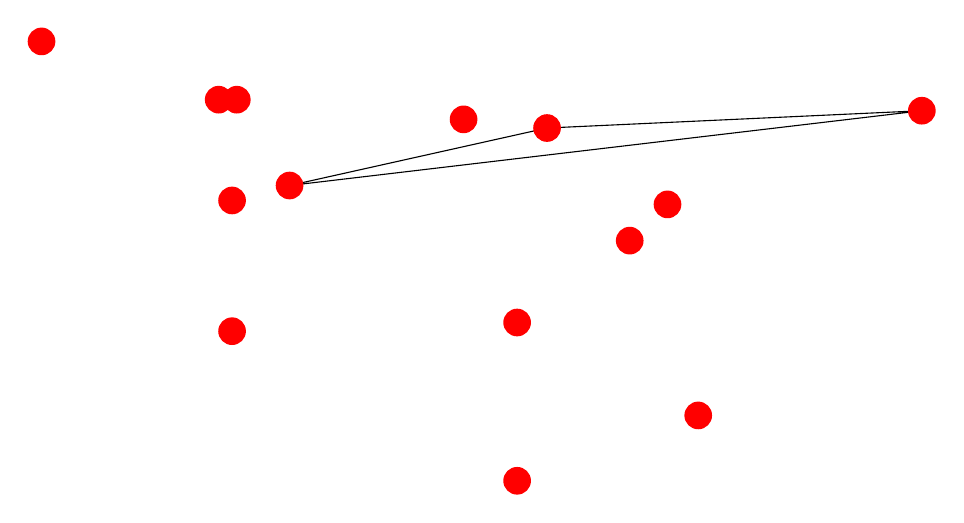
\begin{tikzpicture}
\path   (16.47, 96.10) coordinate (1) {}
        (16.47, 94.44) coordinate (2) {}
   		(20.09, 92.54) coordinate (3) {}
   		(22.39, 93.37) coordinate (4) {}
   		(25.23, 97.24) coordinate (5) {}
   		(22.00, 96.05) coordinate (6) {}
   		(20.47, 97.02) coordinate (7) {}
   		(17.20, 96.29) coordinate (8) {}
   		(16.30, 97.38) coordinate (9) {}
  		(14.05, 98.12) coordinate (10) {}
  		(16.53, 97.38) coordinate (11) {}
  		(21.52, 95.59) coordinate (12) {}
  		(19.41, 97.13) coordinate (13) {}
  		(20.09, 94.55) coordinate (14) {};
\draw[] (7) -- (8) -- (5) -- (7);
\foreach \punto in {1,2,3,4,5,6,7,8,9,10,11,12,13,14}
	\fill[red] (\punto) circle (5pt);

\end{tikzpicture}
\end{document}
